\documentclass[11pt,twocolumn]{article}

\newcommand{\margin}{0.75in}
\usepackage[a4paper, left=\margin, right=\margin, top=\margin, bottom=\margin]{geometry}

\usepackage[utf8]{inputenc}
\usepackage[numbers]{natbib} 		% Package for IEE Referencing
\usepackage[titletoc]{appendix} 	% Package added for the appendix
\usepackage[dvipsnames]{xcolor}
\usepackage{verbatim}
\usepackage{graphicx}
\usepackage{multicol}
\usepackage{makecell}
\usepackage{hyperref}
\usepackage{adjustbox}
\usepackage{filecontents}
\usepackage{lipsum}
\usepackage{url}
\usepackage{soul}
\usepackage{float}
\usepackage{fancyvrb}


% tikz
\usepackage{tikz}
\usetikzlibrary{calc}
\usetikzlibrary{shapes.geometric}

% pfg
\usepackage{pgfplots}
\usepackage{pgf-umlsd}
\usepackage{pgfplotstable}
\usepgfplotslibrary{statistics}

% For Cisco network images
\newcommand{\cisco}{cisco_images}
\newcommand{\ciscoImageScale}{0.7}

\title{\textbf{Investigating the Security of p$\equiv$p’s Trustwords}}
\author{Aidan Fray\\\\ University of York}
\date{September 2019}

% Changes from Bibliography --> References
\usepackage[nottoc,notlof,notlot]{tocbibind} 
\renewcommand\bibname{References}

%Paragraph settings
\setlength{\parindent}{0em}
\setlength{\parskip}{0.75em}

\newcommand{\pep}{p\texorpdfstring{$\equiv$}{E}p~}
\newcommand{\XOOX}{\Verb+\textbf{X}OO\textbf{X}+}
\newcommand{\XOOO}{\Verb+\textbf{X}OOO+}
\newcommand{\OOOO}{\Verb+OOOO+}

\newcommand{\tally}[1]{%
\begin{tikzpicture}
  \begin{axis}[
    ymin=0,
    ymax=200,
    xtick={1,2,3,4,5},
    width=.8\textwidth,
    height=0.2\paperheight,
    grid,
    xlabel={Phonetic raiting},
    ylabel={Oucurrance}
  ]
    \addplot[ybar, fill=blue] table[ 
        col sep=comma,
        y=occurrence, 
        x=rating] 
    {#1};
  \end{axis}
\end{tikzpicture}
}

% Command to make text green coloured
\newcommand{\comments}[1]{\small\textcolor{OliveGreen}{\emph{#1}}}

\graphicspath{{images/}}

\begin{document}
    \bibliographystyle{IEEEtranN}
    \maketitle
    \textbf{\textbf{
    \emph{Abstract} - \lipsum[1]
}}

    \section{Introduction}

The increasing use of public-key cryptography by instant messaging and secure email means ensuring confidentiality is an ever more important task.

One of the most significant risks to the security of the communication channel is a Man-in-the-middle (MiTM) attack. A MiTM attack involves an attacker impersonating one or both sides of a connection. MiTM attacks can entirely circumvent the encryption as it allows an attacker to read all of the encrypted data. A countermeasure for the threat of MiTM attacks is the verification of each parties’ fingerprint. A fingerprint is a small string of characters that is unique to each key and, thus, can be used to identify.

Fingerprints can come in several different encodings such as Hexadecimal, words, and even procedurally generated avatars. Previous research has shown that the average human can only hold around 7-digits ($\pm 2$) worth of data in their working memory\cite{miller1956magical}. Consequently, this makes the designing of user-friendly schemes a task of utmost importance.

Humans are commonly considered the most vulnerable part of any computer system. Solutions, therefore, have been proposed to remove this manual verification with examples such as PGP's web-of-trust\cite{callas1998openpgp} and Namecoin\cite{kalodner2015empirical}. However, these suffer from user adoption due to perceived complexity. Manual verification is, consequently, left in a difficult position, due in part to proposed solutions needing to sacrifice either usability or security. Therefore, research into improving or creating a more secure and user-friendly fingerprint encoding remains an important task.

One proposed user-friendly scheme is Pretty Easy Privacy's (p$\equiv$p) ``Trustwords''. Trustwords is an implementation of word fingerprint mapping with a emphasis on usability. This claimed increase in usability is achieved by the user comparing a reduced number of words. The intended usability boost, however, comes at a cost of a much larger word list ($2^{16}$ words). 

The project aims to assess the security of p$\equiv$p’s minimum recommendation of four Trustwords\cite{trustwordsHandshake}. Moreover, issues with the dictionary's design, such as the presence of homophones and dual-mapping of words show the potential for possible vulnerabilities.
    \chapter{Background}
\label{cha:Background}

\section{Problem Context}
% Goal of the project? Why am I concentrating on PEP's Trustwords?
The project aims to asses the security of \pep's fingerprint representation "Trustwords". Trustwords aim to sacrifice security for increased usability. The encoding scheme has been designed to assist this by having  the user compare a reduced set of words by about half in comparison to other schemes. To achieve this a larger number of bits are required per word. In this case Trustwords maps 16bits per word providing 65537 different combinations. This is, however, the largest number of bits per words (As show in the Literature Review in Chapter \ref{cha:LiteratureReview}) and pushes the boundaries of a language's usable vocabulary.

This abnormal design choice has not received a security assessment to back up claims. This paper, therefore, aims to rectify this research gap.

However, in order to fully understand the project goal it is important to understand public-key cryptography, the role and functioning of \pep and the role fingerprint comparison has in preventing Man-in-the-middle attacks.

\textbf{TODO:} Maybe research questions here instead of in the literature review

\section{PGP}
Pretty Good Privacy (PGP) is a specific implementation of public key cryptography discussed in the previous section. Its main use-case is for securing message based communications but can also be used for file or hard drive encryption.

Each element of a PGP key is split into what is know as a 'packet'. The 'fingerprint' packet v4 contains a version number, timestamp and the main elements of the keys algorithm (i.e. RSA exponent and modulus) formatted as MPIs\footnote{Multiprecision integers are unsigned integers used to hold large integers such as the ones used in cryptographic calculations.}. This data is then preceded with PGP packet header (used to specify length and version numbers). This is all then utilized as input into the one-way hash function SHA-1 to produce a 160-bit digest.

\textbf{TODO: } Generate an image of PGP v4 fingerprint packet

Each key pair is the exclusive-or of each key's fingerprint, this combined values is then broken down into 16-bit chunks and mapped to words via a pre-defined dictionary.

\begin{figure}[h!]
    \centering
    $KeyFingerprint_{1} \oplus KeyFingerprint_{2} = TrustwordsFingerprint$
    \caption{Creation of the combined Trustword fingerprint}
\end{figure}

\begin{wrapfigure}{r}{5cm}
    \centering
    \begin{BVerbatim}
    [...]
52127 ZYGOTE
52128 ZYGOTIC
52129 ZYMURGY
52130 AACHEN
52131 AARDVARK
52132 AAREN
    [...]
    \end{BVerbatim}
    \caption{Re-mapping position in Trustword dictionary}
    \label{fig:remap}
\end{wrapfigure}

Due to the number of words required ($2^{16}$) alongside the design choice to exclude slang and profanities the english Trustword dictionary requires dual-mapping of a section of words. Approximately 13633/65536 (20.8\%) of words are re-mapped in the dictionary leaving 51903 unique words. The re-mapping is also done on a loop with it remaining alphabetical. Figure \ref{fig:remap} shows the position in the dictionary where this occurs. This predictability within the dictionary will be explored later in the paper.




% Does this need explaining?
\section{OpenCL}

\section{Similarity metrics (Soundex etc)}
    % \section{Related Work}

\subsection{Encoding Schemes}
Encoding schemes are the physical method of encoding used to represent the fingerprint. The most common representation is alphanumerical with either \textbf{Hexadecimal} (0-9/A-F) or \textbf{Base32} (2-7/A-Z). These encoding schemes are the most popular due to their intuitive simplicity and lack of hardware requirements.

Fingerprints can also be encoded using natural language. The fingerprint can be chunked and mapped to a set of words. The same principle can be used to fill placeholders in a pre-defined sentence allowing the simple formation of syntactically correct English sentences. Moreover, other languages can be used such as Chinese, Japanese or Korean, to map fingerprint chunks to characters.

A substantial amount of work has been performed assessing the performance of encoding schemes. Results from this literature consistently show the effectiveness of language-based encodings such as Words or Sentences with accuracies ranging up from 94\% \cite{dechand2016empirical}\cite{tan2017can}\cite{kainda2009usability}. In all cases, these were the best schemes from the sets assessed. The exception to this is the work performed by \textbf{H. Hsiao \textit{et al.}}\cite{hsiao2009study} with Words achieving an abnormal accuracy of 63\%. All of the papers assessed simulated attacks and had minimal consideration for technical details regarding their execution. 

Further research has aimed at creating or improving language based encoding schemes. Work by \textbf{Juola} and \textbf{Zimmermann} \cite{juola1996whole} aimed to produce a word list where phonetic distinctiveness was prioritised alongside, \textbf{Michael Rogers'}\footnote{\url{https://github.com/akwizgran/basic-english}} research detailing a process to map fingerprints to pseudo-random poems.

To our knowledge no research has been performed investigating the unique design choices present in Trustwords. This, therefore, is a promising candidate for further research.
    \section{Design}

\subsection{Attack Design}
\label{sec:attackDesign}
The propossed attack on Trustwords involves generating ``near-collision'' keys. Near-collision keys are keys composed of a set of words that are deemed a match by the similarity metrics.
\\\\
The attack is designed to target a single pair of users and requires recomputation for each attack target pair. Each pair is split into an "Uncontrolled" or "Controlled" key. Uncontrolled is the receiver of the communication, and, thus, the key cannot be altered. The Controlled key is the one we are attempting to impersonate. It is assumed that there is the ability to replace the Controlled key with the malicious option. The uncontrolled and controlled keys can be swapped around, thus, resulting in the possibility to intercept both directions of communication.
\\\\
When attacking, a similarity metric is used to compute a list of possibilities for each position in the target fingerprint. Completing these steps produces a list of fingerprints that can be inserted into a tool designed to hash a large number of keys and search for matches. This aspect of using an extensive list to search for keys massively reduces the complexity of the search.

In summary, the attack steps are:
\begin{enumerate}
    \item Compute all possible matches using a similarity metric on all words in a dictionary (Only needs performing once).

    \item Select a target and allocate ``Uncontrolled" and ``Controlled" key identification.
    
    \item Calculate all permutations of near-collisions for the key pair and produce a list of near-collision fingerprints.
    
    \item Use a list of near-collision fingerprints in the mass computation of keys to find near-collision keys.

\end{enumerate}

\subsection{GreenOnion Design}

The inspiration for the design of this tool was taken from a tool called Scallion\footnote{\url{https://github.com/lachesis/scallion}}. The proposed tool is called `GreenOnion' and is a re-write of Scallion in C++.  The proposed tool differs from Scallion, most notably in its ability to concurrently search for a large number of keys. This is due to the unique addition of a bloom filter. A bloom filter is a probabilistic data structure that allows efficient checking for the presence of an element in a set. It is effectively a vast array of booleans that state whether an element is present. A pre-defined hashing algorithm decides the index in the array. This process is repeated several times with a set number of hashing algorithms ($k$) to populate the array of length ($m$). To check the presence of an element in the set means hashing the target value and checking the indices returned. This data structure, therefore, has a complexity of $O(k)$ regardless of the number of elements in the set. Due to the use of hashing algorithms, there is the possibility for collisions and, thus, the possibility of false-positives. The data structure, however, does not produce any false-negatives. If the levels of false-positives are controlled (by altering $k$ and $m$), the tool can search through a vast number of potential keys with minimal decrease in speed.

The tool should take two keys as parameters (Uncontrolled/Controlled) and a chosen similarity metric and produce a list of target key fingerprints. This list is then used as a search criterion when searching for keys. To utilise the parallel nature of the GPU to compute the hash of a large number of keys, the tool utilises a GPGPU (General-purpose computing on graphics processing units) framework. OpenCL allows the creation of code chunks referred to as ``kernels'' to be executed concurrently, this provides a massive speed increase compared to the sequential nature of the CPU.
    \section{Experimental Design}

\lipsum[3]
    \section{Results}


\subsection{Scallion vs GreenOnion}
\label{sec:SvG}

This section compares Scallion and the newly designed GreenOnion ability to search for a large number of potential keys.

Figure \ref{tab:scallion_speed} shows the speed decline as the number of concurrently checked potential keys increases. Alongside the results for base version of Scallion is the speed for \textit{Scallion Improved}. This is the same Scallion code but with a fix that reduces the severity of the speed decline. Scallion contained a call in its print statement that became become increasingly expensive as the number of concurrently checked keys increases. Removing this line from the print statement results in a sizeable improvement in speeds as can be seen in Figure \ref{tab:scallion_speed}. This was necessary to include as we believe the improved versions show a better comparison between the design of the two tools. 

\begin{figure}[h!]
    \centering
    
\begin{tikzpicture}[every axis plot/.append style={thick}]
    \begin{axis}[
        width=\linewidth,
        height=10cm,
        grid=major,
        xmin=1, xmax=40,
        % ymin=0, ymax=100,
        xlabel=Number of Keys,
        ylabel=Hashing speed (MH/s)
        ]
        \addplot table [x index=0, y index=1, mark=none, search path=data, col sep=comma]{scallion.csv};
        \addlegendentry{Scallion}
        
        \addplot table [x index=0, y index=1, mark=none, search path=data, col sep=comma]{green.csv};
        \addlegendentry{GreenOnion}	
     \end{axis}
\end{tikzpicture}
    \label{tab:scallion_speed}
    \caption{Speed comparison between Scallion and GreenOnion}
\end{figure}

GreenOnion's speed is almost perfectly consistent. It is slower up until  around 800 keys. This initial lower speed is due to the overhead of the bloom filter; however, as the number of keys increase, the bloom filter's benefits become apparent. In this test, the bloom filter size was kept consistent at exactly 10,000 elements. 

Scallion was unable to handle anything over 2513 concurrent keys. This was due to the search strings being passed via a command-line argument as a regex string. This number of keys hit the character limit of a Powershell command. GreenOnion, however, has been tested to handle more than 1.5 million keys with a slight reduction in performance. This improvement over Scallion is, therefore, substantial. GreenOnion's code has been made publicly available and can be viewed on GitHub\footnote{\url{https://github.com/AidanFray/GreenOnion}}.

\subsection{Experiment 1 - Metric performance}

The goal of this experiment was to select a set of metrics to be assessed in the subsequent experiment. This section discusses the demographics of participants alongside the subsequent results.

% \subsubsection*{Demographics}

Overall, 104 participants were assessed in this study. Five results were discarded from the set due to either failing the attention questions (See in Section \ref{sec:exp1_qualitycontrol}) or having too low of a fluency rating. This dismissal was a necessary process to improve the health of the results. 

Table \ref{tab:exp1_demo} contains the demographical breakdown of the reduced set of participants. The average ages of the participants were 37.3 years ($\sigma = 11.67$) with a split of 44.4\% of Males to 55.6\% of Females. As can be seen, over 60\% of participants can be considered highly educated (Bachelor’s and up). This level of education is not sufficiently reflective of the general population and therefore, has to be considered when interpreting the results. All participants were sourced from the US; this again requires consideration due to the broad range of dialects present that may bias the results. Further work could investigate the effect of location and dialect on similar results. 

\begin{table}[h!]
    \centering
    \begin{tabular}{|l|ll|}
        \hline
        Gender & Male: & 44.4\% \\
               & Female: & 55.6\% \\
        \hline
        Age:   & 18-24: & 10.1\% \\
               & 25-29: & 20.2\% \\
               & 30-39: & 31.3\% \\
               & 40-49: & 21.2\% \\
               & 50-59: & 12.1\% \\
               & 60-69: & ~~4.0\% \\ 
               & 70-79: & ~~1.0\% \\ 
               
        \hline
        Highest Education:  
        & GCSE:                 & 13.1\% \\
        & A-Level/O-Level:      & 19.2\% \\
        & Bachelor's degree:    & 52.5\% \\
        & Master's degree:      & 13.1\% \\ 
        & PhD:                  & ~~2.0\%  \\
        \hline

    \end{tabular}
    \caption{Participant demographics}
    \label{tab:exp1_demo}
\end{table}

Figure \ref{tab:exp1_results} shows the average results for the selected matches. It can be seen that Levenshtein came out substantially above the rest. Levenshtein also has a much more significant proportion of 4 and 5 ratings than the alternatives.

Due to the averages of Metaphone and Phonetic Vectors being so close standard deviation was used as the final decider. As can be seen, Megaphone has a slightly lower $\sigma$ value of that of Phonetic vectors, thus, contributing to the decision to select Metaphone.

\begin{table}[h!]
    \centering
    \begin{tabular}{|l|l|l|}
        \hline
        \textbf{Metric} & \textbf{Average Rating}  & \textbf{$\sigma$}\\
        \hline
        Leven     & 3.66  & 1.15\\
        NYSIIS    & 2.92 & 1.31\\
        Metaphone & 2.56 & 1.32\\
        Phonetic Vec & 2.50 & 1.35\\
        Soundex & 2.08 & 1.12 \\
        \hline
        Random  & 1.16 & 0.46\\
        \hline
    \end{tabular}
    \caption{Average metric performance}
    \label{tab:exp1_results}
\end{table}


%TODO: Include graphs?

\subsection{Experiment 2 - Trustword attacks}

\begin{table*}[t]
    \makebox[\textwidth][c]{
        \centering
        \begin{tabular}{|ll|l|l|l|}
            \hline
            \textbf{Metric} & & \textbf{Successful Attacks} & \textbf{Total Attacks} & \textbf{Success Rate} \\
            \hline
            Levenshtein && 218 & 1101 & 19.8\% \\
            \hline
            & \OOOO   & 34  & 358  & ~~9.5\% \\
            & \XOOO   & 59  & 353  & 16.7\% \\
            & \XOOX   & 125  & 390  & 32.1\% \\
            \hline\hline
            NYSIIS &&  209 & 1114 & 18.8\% \\
            \hline
            & \OOOO   & 36 & 385 & ~~9.3\% \\
            & \XOOO   & 72 & 375 & 19.2\% \\
            & \XOOX   & 101 & 354 & 28.5\% \\
            \hline\hline
            Metaphone &&  181 & 1072 & 16.9\% \\
            \hline
            & \OOOO   & 38 & 345 & 11.0\% \\
            & \XOOO   & 57 & 375 & 15.2\% \\
            & \XOOX   & 86 & 352 & 24.4\% \\
            \hline\hline
            \textbf{Overall} & & 608 & 3287 & 18.5\% \\
            \hline\hline
        \end{tabular}
    }
    \caption{Success rates for simulated attacks}
    \label{tab:exp2_attacks}
\end{table*}

\label{sec:exp2}
This experiment aims to quantify the success rate of the proposed attack. Design details for this experiment can be seen in Section \ref{sec:exp2_design}. This section presents and discusses the results of the experiment alongside a comparison to relevant literature.

Overall, 435 paid participants recruited via Amazon's MTurk were assessed in this experiment. We excluded 66 results; 7 due to being non-native speakers and 59 were discarded for failing the attention metrics (Discussed in Section \ref{sec:exp2_quality})

\begin{table}[h]
    \centering
    \begin{tabular}{|l|ll|}
        \hline
        Gender & Male: & 50.4\% \\
               & Female: & 49.6\% \\
        \hline
        Age:   & 18-24: & 12.7\% \\ 
               & 25-29: & 18.2\% \\ 
               & 30-39: & 37.4\% \\ 
               & 40-49: & 17.9\% \\ 
               & 50-59: & ~~8.7\% \\ 
               & 60-69: & ~~4.3\% \\ 
               & 70-79: & ~~0.8\% \\ 

        \hline
        Highest Education:  
        & GCSE:                 & 13.8\%  \\
        & A-Level/O-Level:      & 24.1\% \\
        & Bachelor's degree:    & 51.5\% \\
        & Master's degree:      & ~~8.4\% \\ 
        & PhD:                  & ~~2.2\% \\
        \hline

    \end{tabular}
    \caption{Participant demographics}
    \label{tab:exp2_demo}
\end{table}

The reduced set of 369 participants had an average age of 36.6 ($\sigma = 11.35$) and consisted of an almost equal split of Male (50.4\%) to Female (49.6\%). Around 62\% of participants had completed a single stage of university (Bachelor and up). This aspect makes this set of participants more educated than the general population. All participants were also sourced from the USA and have rated themselves as fully native English speakers.

Table \ref{tab:exp2_attacks} contains the break down of results for the experiment. It can be seen that the best metric out of the set was Levenshtein with an overall success of 19.8\%. The best performer, when regarding attack strength, as expected, is the \XOOX~attack. Levenshtein's \XOOX~attack performed the best overall with a success rate of 32.1\%. The worst performer was Metaphone, with an average of 16.9\% over its three levels of attacks. When comparing the performance of the metrics to the previous experiment, the ordering remains the same with Levenshtein, NYSIIS and Metaphone all ranking in the same order.

\subsection*{Comparison to alternative literature}
This section compares the results of the experiment to similar literature.

Work by \textbf{R. Kainda, I. Flechais} and \textbf{A. Roscoe}\cite{kainda2009usability}  is the most comparable to this experiment. They were the only study to use exactly 4 words but differed on the size of the dictionary (1024 words) and how a near-match were calculated. Near-matches were a difference in a single word, but without the consideration for similarity, this is the unique aspect considered with this experiment. However, with those aspects in mind attacks on words encoding received an overall success rating of 3.3\%, considerably lower than that of this study. In the worst-case, our simulated attacks achieved almost 3 times as many successes compared to this study.

Other relevant work by \textbf{S. Dechand \textit{el al.}}\cite{dechand2016empirical} assess the success rate of attacks on words. Their experiment is less similar as 14 words per attack were assessed with each participant, where the comparison was performed visually. However, the success was 8.78\%. As 10/14 words were kept static, this result is more comparable to the highest attack strength (\XOOX). This, therefore, leads to another 3 fold improvement in the success rates of our simulated attacks. 

The final relevant paper to compare is that of \textbf{J. Tan \textit{et al.}}\cite{tan2017can}. This paper had the highest number of words assessed with 16 overall. With it assessing the same wordlist and attack strength as the work by \textbf{S. Dechand \textit{et al.}}\cite{dechand2016empirical}, the attack success was 14\% overall. This success rate compared to the highest attack assessed in the experiment results in another sizeable difference.

In conclusion, all related literature had much lower attack success rates that the results presented in this experiment. With all papers using similarly designed wordlists, it highly suggests that the deficiencies in Trustwords are the cause for the substantial increase in attack success. Alongside this, the consideration for similarity when calculating near-collisions could have also resulted in the higher attack success rates. This aspect is also a unique consideration compared to the available literature.
    \section{Discussion and Further Work}

\subsection{Further work}

\subsection*{Trustword improvements}
The first area of proposed work could be recommendations into how to improve Trustwords backed by empirical evidence. We feel the most promising avenue would be the utilisation of Phonetic Vectors unique qualities to identify words of low quality by measuring very low vector distances. For example, present in the dictionary are the words \verb|THERE| and \verb|THEIR|, these could be massively improved upon and could result in a better quality word list. Moreover, utilising the quantification of dissimilarity could be used to create a dictionary of maximized phonetic distance. This phonetically distinct wordlist could then be assessed in a similar way with its success rate quantified against users.

\subsection*{Similar metrics performance}
Another area of further work is the comprehensive assessment of algorithms used to assess phonetic similarity. The algorithms assessed in this work are a very small proportion of potential options. Thus, further work could assess the performance of metrics against each other to determine the one that works best with human models. A conclusion could be reached by running the improved experiment discussed in Section \ref{exp:metric}, where it could be repeated with an increased number of metrics. Other elements for consideration could be age, location and dialect as variables that affect a metrics performance. 

\subsection*{GreenOnion optimizations}
A minimal amount of work was allocated to improving the performance of GreenOnion as low-level optimizations are very time-consuming. A project, therefore, could aim to improve on the performance already recorded in this paper. This project could improve the performance of the attack and allow for more effective keys to be computed in less time. 

\subsection{Conclusion}
Overall, the project has demonstrated a potential attack on \pep's implementation of Trustwords. An attack was proposed that utilised phonetic similarity algorithms to exploit the weaknesses in the Trustword dictionary to generate near-collision keys. To achieve this, a tool was created to compute a massive number of keys concurrently. It was based on a known tool but improved substantially on its key searching performance. The performance of similarity metrics was compared alongside an experiment assessing participants fallibility to the proposed attack. Results showed as much as a 32.05\% success rate for the best attack. The main project aim was to show that the recommend minimum number of four Trustwords was insufficient to provide a basic level of security. We believe we have demonstrated that four Trustwords is too low to provide enough security for general use-case and the minimum provided words should, therefore, be increased.

    \bibliography{references.bib}
    
    \appendix

\chapter{Randomly generated uncontrolled key}
\label{appendix:uncontrolled_key}

\begin{lstlisting}
-----BEGIN PGP PUBLIC KEY BLOCK-----

mQENBF0vHaYBCACxOy7RacHIprgaUo66vGmIB2VIaSwToliuaEBxOAloD+wTB/T9
TOKgAMLWMgK2z3/tOZj2l5k9ATUr0nZ9iBgew5Ih3ykOp+OkE9dh4NTD3EJz5UWo
M1r6scPhby92zMBqKi0iPFlPcvk+eg+SPusxIp+Vn16ALoB2pwGQvG+qoFEJfdVP
nwSAWJo1mcd+TCxgIMqe11FXDzxpd4BEpMXsHOB8NH/TUiI57sxqT8A2HnnyWo2i
5vs93VAP8rTTIRfGelW2c3oqhV9XhXbvVpJPmvkTxM/SshV1L5HhYr1TUAkAQw6w
RUZqooysgZEDqQw58lFQ7C9plCHOpXIEhbE7ABEBAAG0HEpvaG4gSm9obnNvbiA8
am9obkB3b3JrLmNvbT6JAVQEEwEIAD4WIQRQZ0ukmi5QUEz7KB3FwHKSVKqpwgUC
XS8dpgIbAwUJA8JnAAULCQgHAgYVCgkICwIEFgIDAQIeAQIXgAAKCRDFwHKSVKqp
wg4YB/9knveazSM4yN3EJY7HRZe5PVA5r0GGDlEDMte+surPKLsV/T39SNl8qTH+
DXnOyC4rt1kykTJP+ULcKqGkVRnH2XYZP/W6E9wwBPjoKHaWyn8MP0ix5kgkq6Ld
ZWEQ2pUwCsAhWv8K/ybjQ+Li484JKbrz/GRALp8qU3hZgCo/Fw3sD2KcTPU1v8qU
av9G2N5su10W7G0F1ozszFit+r2iinoZtGSddBPG+pIUEtZoBn4V2FRRSO1UY/TU
jGf2BLsk+ZkNJdx5x6IEU9CQ+ivPuKtupVu9ySKqE2Qfmn5lh9iAjYDN3XxUQfCf
braGoC9JLnL5QmT1JaQXfxkIHilyuQENBF0vHaYBCADDp/u8D/TG5d5HmabmgbBF
3R2d3J00vt7VQQ5sIRMLyP0cx6qy2bTIy9mgfU3/WcrhRp728gBo+NnUfxyiTb5R
u7AbntlkerF3dh0JLm5eIossPW37QXn3Ce4Tv4ixGRLbsGKTu6h0lP41FM5VcqV9
9NE1iml3WyngnsFdKeUYqPW4QY+ydyjpSyblbQTMptIKG2llCmsd9k+hb8nnGx/d
GvyGKaZ270iVGY2im/9VP2VwzqXlFxxx6Dux4egJJMMAy5xkzBKf+Szmm1pMJkt2
4sBrwmLnuUObgsAkq8K+MqEpWeFi6aWsh7RnY8T0SEb/3QUwG12V77ePhrarBwmf
ABEBAAGJATwEGAEIACYWIQRQZ0ukmi5QUEz7KB3FwHKSVKqpwgUCXS8dpgIbDAUJ
A8JnAAAKCRDFwHKSVKqpwoW3CACeKIcQFuVv2vpUHq/4ATH0atPYqR1NbJTegE+v
XZyrNHtmRF4V+kdx/1KX9jsIY2TjyxbhTsrtMFkMZMfAVjXVoS4y8OkwX5IJWgHC
0JQIHQrvaIGfI1yuVrNvWYyPXFxNtbntrgTd8JKYGKYaTqXNZ2r1ozbZElp7fQtR
rWNUGJYYo+aHHLM+Aot5k+Z3YqHifuPSnCEYt/GxnMhYq1IL3LSZ96hsgwqeFoLP
+v4RsvY52Yb5tiOzxZwikALOJdM2aAumxq8R1nYHiswWxotw2WkKFlB7gfLpbMWs
Y+o4J7QKSqpVTrUYBTPF1F4kBWOMY10kpeCDbZ1YwJOZJf8P
=aHBu
-----END PGP PUBLIC KEY BLOCK-----
\end{lstlisting}

\chapter{Computed Attack Keys}

\section{NYSIIS - 0 Static}
\label{appendix:nysiis_0_static}

\subsection{Controlled Key}
\begin{lstlisting}
-----BEGIN PGP PUBLIC KEY BLOCK-----

mI0EXS8lIAEEAMWEJ+NGB/ukiUijzdT+DvzVwouWV/j4Rw78X9YdgJP0ExT4ncHG
TJbOKjEMEI9bb/oYMLF/434ufScYNci+rL/3RVY8CcjEv5l0UGX+udZ78c7Z/vf1
zFr2MQAglr9M8599JwUY25LiNKzDYc87B16hqRV8hRaXHfAFFHBxRsgBABEBAAG0
HUF1dG9nZW5lcmF0ZWQgS2V5IDx1c2VyQENWRUQ+iNQEEwEKAD4WIQSlBU278MbT
iVM5h6GNohojnp5YQgUCXS8lIAIbLwUJAeJfkAULCQgHAgYVCgkICwIEFgIDAQIe
AQIXgAAKCRCNohojnp5YQvxSA/0bjL+4me3hLjrM+8IckKABCRdRYYRG7svbln9q
ULUngsXMpbIMoHFg1ePpT2lniiHtQhDC88ZW1J5yeVZN1cfJhRsByyKlkzG3Dcy7
5wKonbVz1LSYpIDq/DNNP0eINzuVNc1rxqRXPGAh6NHnmZN5MqxLNyu0DSX9oJHm
KbbtLQ==
=FQCu
-----END PGP PUBLIC KEY BLOCK-----
\end{lstlisting}

\subsection{Computed key}
\begin{lstlisting}
-----BEGIN PGP PUBLIC KEY BLOCK-----

mQEOBF0zhx4BCAD0iC55GShgArPzKZdn6we2mrkxS8o8fI7HdWXnLoRAta1Q1j9z
U+mYU9tGYb0yjqIARjjUK2qnq0CsGZJpB65AhbrOsDLv6dmI68tuiT4xjmzcM6+6
6M/EY5E5hYpZeurDJ8rSYrfu/v9P0bV78VnM17uUl4PTyEBmbJsE9kszq4MXd5yz
G+ibBPBvnBWSlRQzyCFMgTL8gQH36XJUj7jgxTKoJWzli/QtNcMOjwSQtEZxFWVK
+qsJjYUClpg9Kkow1LqJmEc1Tj98EipypDtdwNQhn4wHQVgu7SliaNNmrR8MpP9o
gL9hhfafx5FsE7v4zHhzu+ubR+c7KnUlwJyfABkBhI5atQAeSm9obiBEb2UgPGNo
YW5nZV9tZUBlbWFpbC5jb20+
=
-----END PGP PUBLIC KEY BLOCK-----
\end{lstlisting}

\newpage

\section{NYSIIS - 1 Static}
\label{appendix:nysiis_1_static}

\subsection{Controlled Key}
\begin{lstlisting}
-----BEGIN PGP PUBLIC KEY BLOCK-----

mI0EXS8o2AEEAKQmxot2Z5XFrNjg4zXBfvLsTzoO3vZeEI9l8+U2X8aq5KVQJpPU
BRSfqQuMZvA1zh3vH3w4I/vR4nXCNw/hPCi0B/DckUe6IJPZJfMiQfT1Xt16ZEms
W53CBiNqnt5xruo4wKwoKGuHELtPcD4K/iBIFt6n3UTi+R8xU4WMc+PjABEBAAG0
HUF1dG9nZW5lcmF0ZWQgS2V5IDx1c2VyQENWRUQ+iNQEEwEKAD4WIQTFXc8VXOqe
13ib81dcbeH3Z8A13wUCXS8o2AIbLwUJAeJb2AULCQgHAgYVCgkICwIEFgIDAQIe
AQIXgAAKCRBcbeH3Z8A13wItA/kBbfc6kxtLumDQiGpcIzgWmM9UhCn0V8ny9iB2
gt4V8bImpC3qicj6+KywsEsvFIgsJO0UcNeoREKanpXxPf6T7tvBUTLQjPJFedsn
J57996JiZ9COQ4lEg2AvfAKy1alKrMs0Xy4hWrHY9cJWs1a7KpbrsioHd4vDRgMS
2yRn/w==
=krrv
-----END PGP PUBLIC KEY BLOCK-----
\end{lstlisting}

\subsection{Computed key}
\begin{lstlisting}
-----BEGIN PGP PUBLIC KEY BLOCK-----

mQEOBF0yA4QBCAC78Lk2k9BdUEufpqll4D60iAuYVrxVs3lpjwP2hpztBFFw8vY4
26uW1C7MPo9l4Oteks5626hwAAgI1/YHFwWpBDdTWYEnVGrjv5v0Juz5IZc7kiwp
Ui2XWJ7I3VpE5nljFyzaQMGaS5Cvmtco5cjin1Tx486jieGBt0loQQdtiJ3gEAFT
XlUvwIQSdYWY2F8xWKg5aJoDFEZN74KfwQqB7hx/53VHyzOJGygnvvpMcJaX3c8E
V3t7n90WvXJWND7bn6HIJrnFKyRJsKHneL2n0wGd/N0NLCuLTvNK+uQ7sXGNZox1
Qa4a1guiSdaq9NO5mX+tOYox3/onzpshJgVDABkBvckntQAeSm9obiBEb2UgPGNo
YW5nZV9tZUBlbWFpbC5jb20+
=
-----END PGP PUBLIC KEY BLOCK-----
\end{lstlisting}

\newpage

\section{NYSIIS - 2 Static}
\label{appendix:nysiis_2_static}

\subsection{Controlled Key}
\begin{lstlisting}
-----BEGIN PGP PUBLIC KEY BLOCK-----

mI0EXS8s+gEEANkph53UuQkNVFhYimrzH0bXBp/Y3InV9p5MP09TZxtTOf44JBPp
MCFMvgFJpVK3D5PQ2h7fW1lNb41THkiGC7Jk+F7gd+beqH5kaaKmC+RNAF0aZ5av
2al5JvtHT0Z8/1r8bxfp33WLmQXK0/9EwL4HvERRGh7wZ5WemvCrvZPXABEBAAG0
HUF1dG9nZW5lcmF0ZWQgS2V5IDx1c2VyQENWRUQ+iNQEEwEKAD4WIQSjUV9vxlLP
LPE78Z2TulybLqhYHAUCXS8s+gIbLwUJAeJXtgULCQgHAgYVCgkICwIEFgIDAQIe
AQIXgAAKCRCTulybLqhYHONrBAC8uh/K2Adq/o/Qe/EVM5JpT6ETE1WlAj2iUMWB
MAmdjgiQlRyBCTd4Lt9xFsbnvQG9pj4GVHosXjVpuA/1NxyS+DE4EkBDzXA3NuR8
0djhyD27VSsn2q1j8bB1wxO7sLbjo30SIBG2wUaft5DVJiBGG69kh4pt+aKKOcjb
LLPldw==
=dCl/
-----END PGP PUBLIC KEY BLOCK-----
\end{lstlisting}

\subsection{Computed key}
\begin{lstlisting}
-----BEGIN PGP PUBLIC KEY BLOCK-----

mQEOBF0wxGEBCACsqQN92G3IizweQHw42OhUM5ZySKTvzPqVhAeCb2ETSBDZFbGN
lHYPa6dytXwLbU6kdlt8kgxbk75iPJsCSPLAUzKvlVd2rkTu5xtKPFqDTRvbjOjf
Ik8zJimXJGZNYVrMUqkfPR2FtVC4VUJXtML8voj/1lcLxTWRcYjuNQuSRNhJQtUP
ViZMTj97IO894lVg+ciZXEZkzHzlriqeLqwTupQxvzqjmObmeH1NCPSfGcTSNIBu
cNG/DrXTXsVpZPUilIRsXTtc2FM9iY49Zjv01KdzsJlV97JVyghYFFCEe1xq7Twp
U9TOzypXD4NdTKivFZUNT4jdG2HoJE4IcZ3NABkBh0qYtB5Kb2huIERvZSA8Y2hh
bmdlX21lQGVtYWlsLmNvbT4=
=0nU6
-----END PGP PUBLIC KEY BLOCK-----
\end{lstlisting}

\chapter{Trustword Attack}
\label{appendix:trustword_attack}
\begin{figure}[h!]
    \centering
    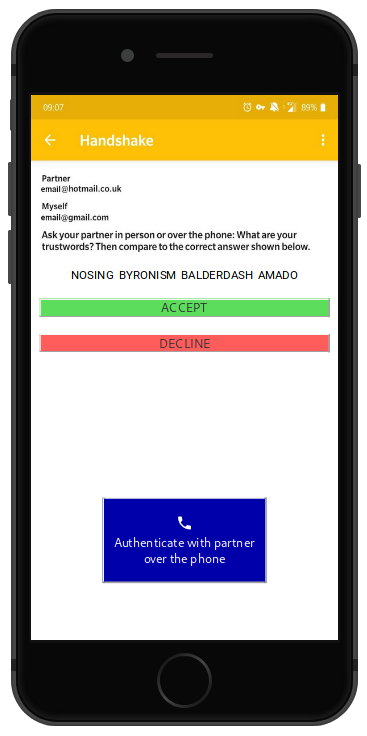
\includegraphics[scale=2.5]{experiment/trustword_attack.png}
    \caption{Experiment UI}
    \label{fig:expID}
\end{figure}

\end{document}
